\newpage
\section{Metodologia Experimental}

    \subsection{Materiais}
        O material utilizado para realização do experimento foi:

        \begin{itemize}
            \item U-2970A Gerador de dados;
            \item U-2970B Formatador de dados;
            \item U-2970C Modulador balanceado duplo;
            \item U-2970F Regenerador de clock de dados;
            \item U-2970G Recuperador de dados;
            \item U-2970H Receptor de dados;
            \item U-2970K Módulo de áudio;
            \item U-2970M Fonte de alimentação;
            \item U-2970N Conjunto de cabos de alimentação;
            \item 1 Osciloscópio de 2 canais.
        \end{itemize}

        Para execução do experimento, faz-se necessário executar os passos a seguir.

    
    \subsection{Método para regeneração do clock}
        \begin{enumerate}
                \item Realizar a montagem do equipamento de acordo com a Figura \ref{fig:m1}, utilizando o módulo de áudio como saída (ligações 23 e 24).
                
                \item Configurar os canais 1 e 2 do osciloscópio com acoplamento DC, escala de tensão 5V/divisão e base de tempo  10$\mu s$/divisão, com trigger externo na borda de clock da palavra.
                
                \item Conectar o canal 1 na saída NRZ do módulo U-2970B e o canal 2 na saída bi-fásica, verifique que o sinal está atrasado de metade do tempo de bit quando comparado com a entrada NRZ.
                
                \item Utilizar a entrada de dados para produzir vários padrões de bit, observando como o código bi-fase é relacionado aos dados básicos. Observe que, na primeira metade de cada período  de bit, o sinal bi-fásico corresponde ao bit original e na segunda metade ao inverso do bit original.
                
                \item Note que para a produzir a saída bi-fásica é utilizado um clock com frequência de 80kHz para trocar a polaridade do sinal durante a segunda metade do tempo de bit (ligação 12). A negação é realizada pelo modulador e o clock de 80kHz deve ser sincronizado com os dados de entrada.
                
                \item Um enlace de comunicação é estabelecido pela ligação 7 e 8, agrupando o transmissor (saída bi-fásica do módulo U-2970B) ao receptor (entrada do módulo U-2970F). Para garantir a uma transição precisa na ligação 11, um dado quadrado é empregado.
                                
                \item Mover a ponteira do osciloscópio para a ligação 11 e o soquete para a sua direita. Observe que um pequeno pulso é gerado em cada transição do sinal quadrado, produzindo um pulso de sincronização é gerado no centro de todos os períodos de bit, porém, somente algumas vezes entre os períodos de bit.
            \end{enumerate}
            
            \begin{figure}[H]
                \centering
                \caption{Montagem do equipamento para geração do código bi-fase.}
                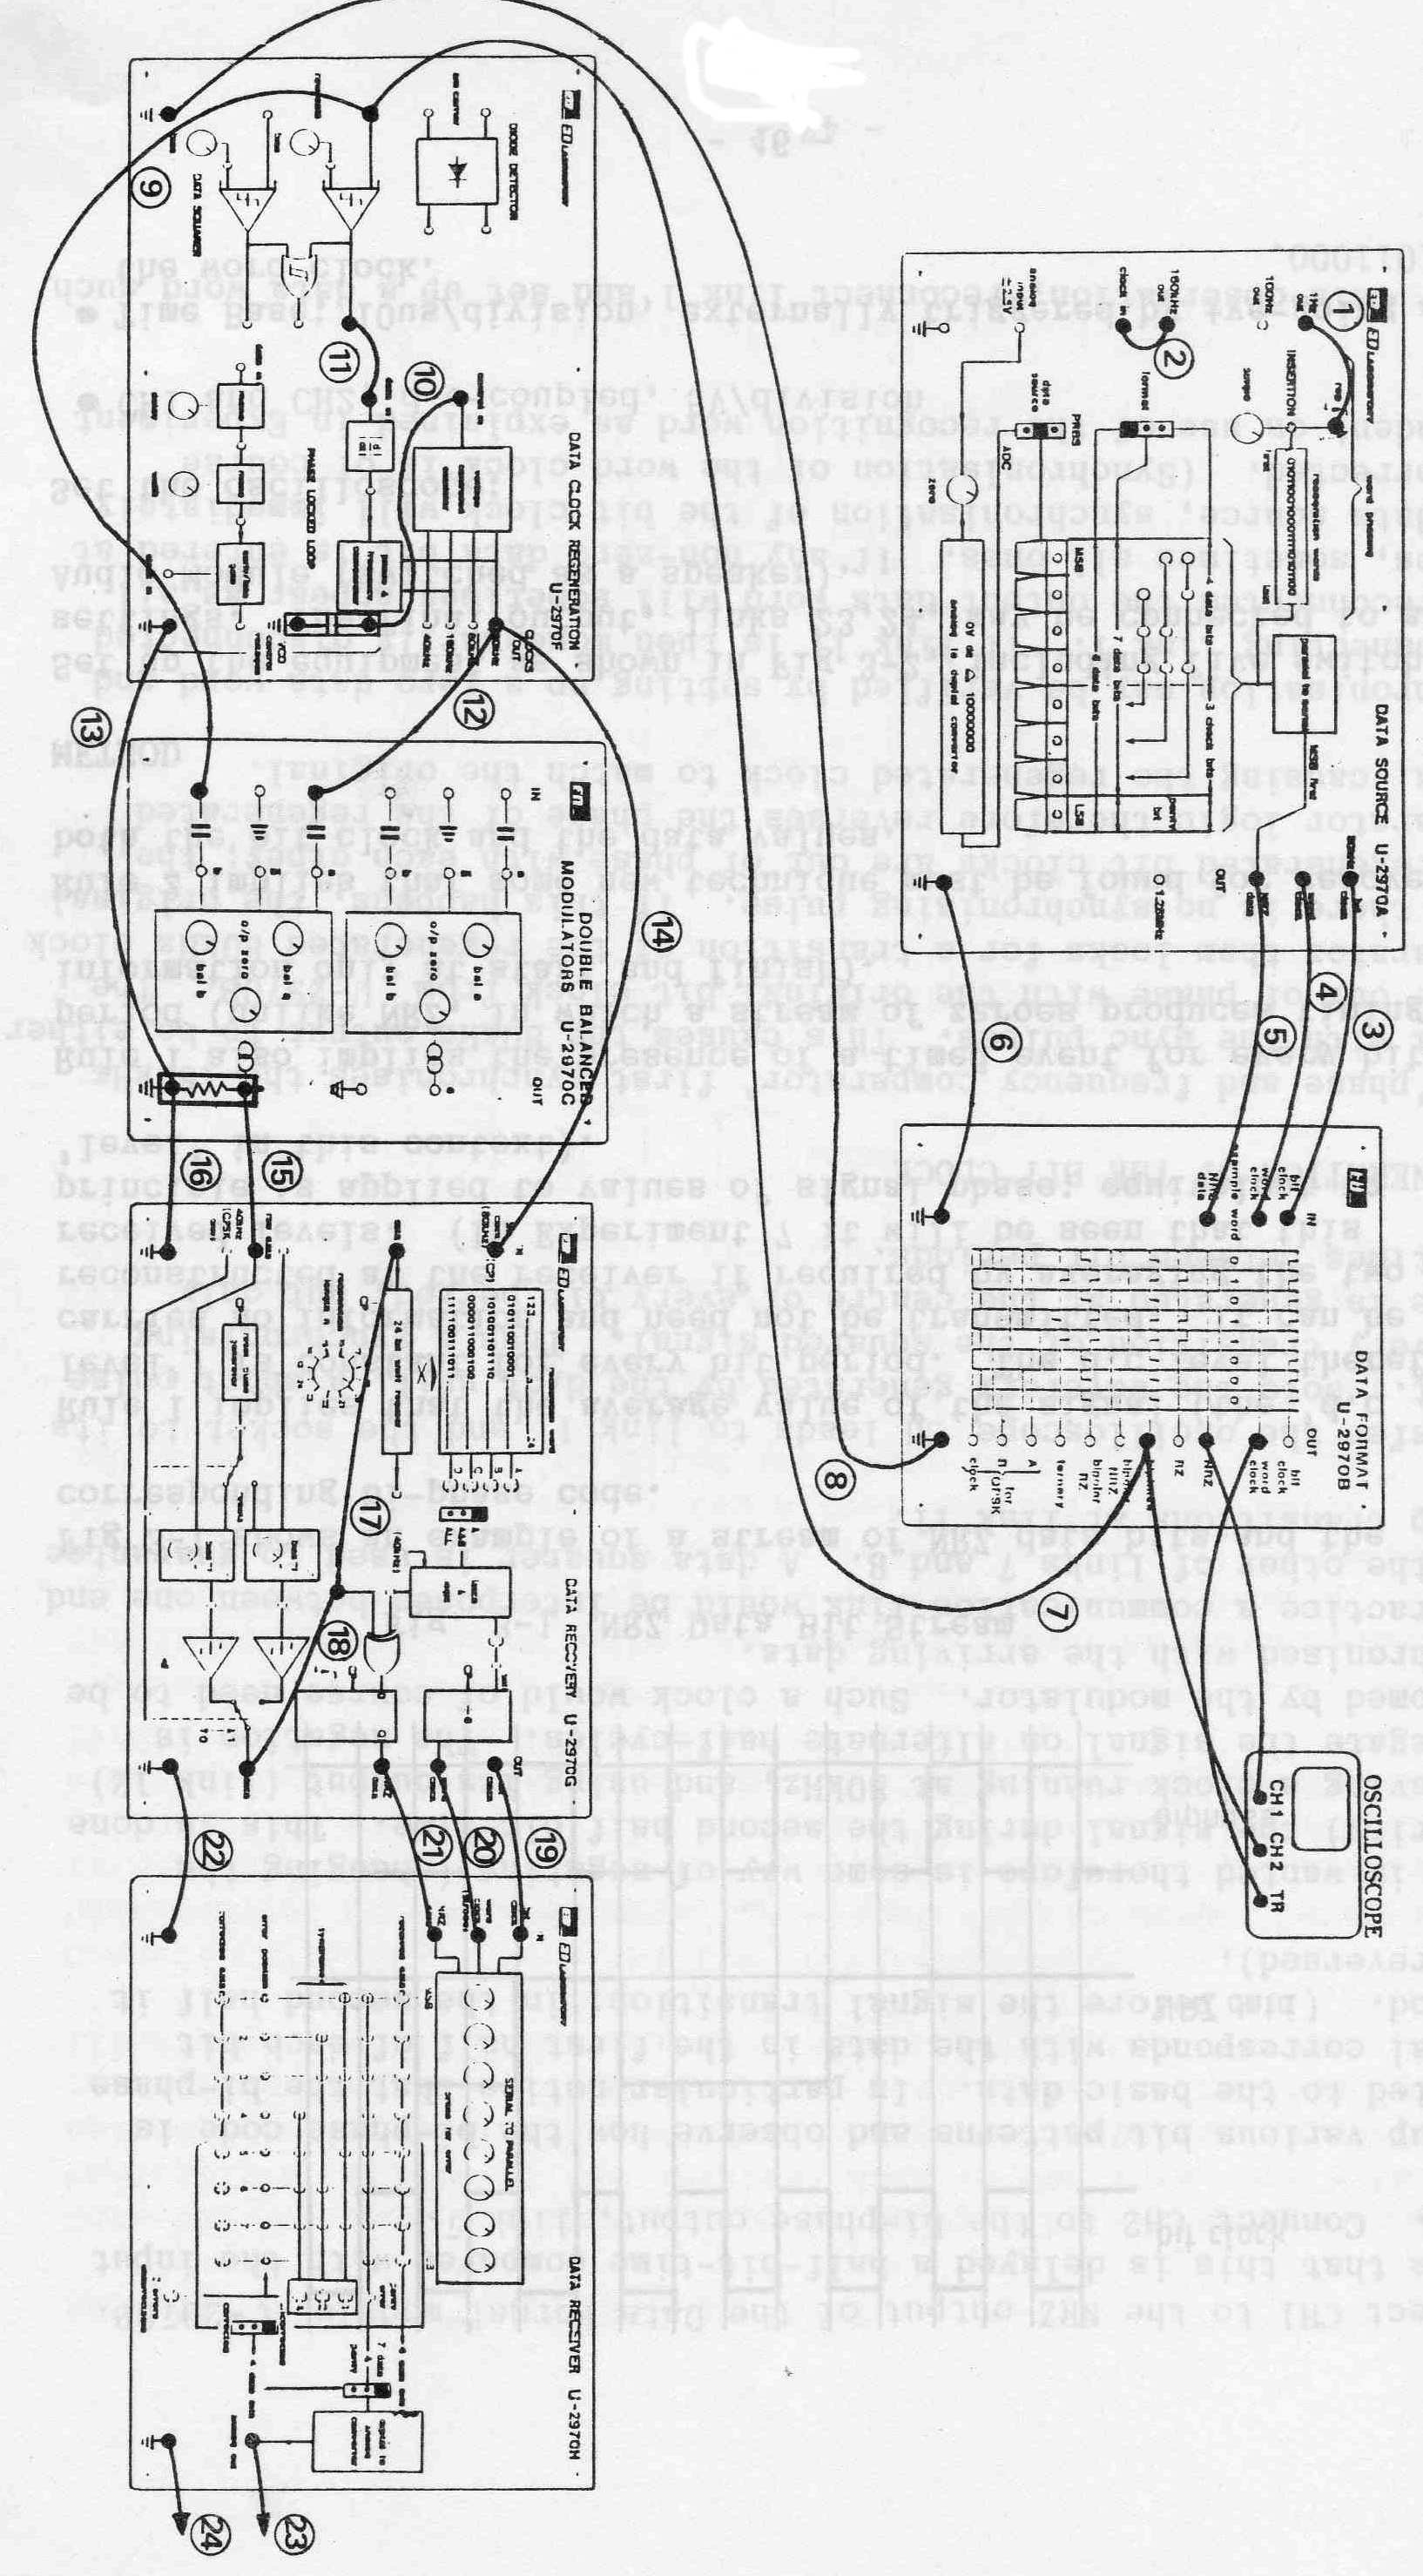
\includegraphics[scale=0.18]{m1}
                
                \small Fonte: Jacob, J. L., Roteiro de laboratório, 2017.
                \label{fig:m1}
            \end{figure}
            
        \subsection{Recuperação do bit de clock}
                        
            \begin{enumerate}
                \item Verificar a sincronização configurando uma palavra de dados zero e desconectando a ligação 1.
                
                \item Quando a ligação 11 é desconectada momentaneamente e reconectada, a a palavra de dados de saída aparecerá hora tudo zero, hora tudo um.
                
                \item Caso um dos bits de dados seja 1, haverá a sincronização do bit de clock imediatamente.
                
                \item Reconecte a ligação 1 e configure a palavra de dados como 01011000.
            \end{enumerate}
            
            
        \subsection{Recuperação dos dados}
            \begin{enumerate}
                \item Para verificar a recuperação dos dados, ligar a ponteira do canal 1 do osciloscópio na ligação 15. A forma de onda deve ser basicamente uma réplica dos dados originais (NRZ), porém, com grandes picos sobrepostos. Visto a existência de grandes picos sobrepostos, a técnica \textit{integrate and dump} é empregada para a recuperação dos dados, conforme mostra a Figura \ref{fig:integrate}.  
                
                \item. Mover o canal 2 do osciloscópio para a saída do integrador utilizado e ajustar o potenciômetro de modo a obter uma polarização adequada. A saída do integrador deverá mostrar que a saída cresce durante um bit 0 e decresce
                durante um bit 1. Ao final do tempo de bit, o integrador é zerado para o início de um novo bit.
                
                \item Note que os picos de curta duração observados no canal 1 possuem pouca influência no nível do sinal no canal 2.
                
                \item Note que o sinal do de saída do integrador, mesmo com picos de amplitude, é suficiente para representar os dados.
                
                \item Os dados recuperados podem ser observados passando o canal 1 do osciloscópio para a ligação 17.
            \end{enumerate}
            
            
         